\begin{figure}[h]
    \centering
    \addletter{115}{a}
    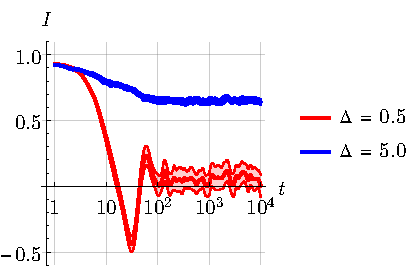
\includegraphics{imgs/2Dth_loc.pdf}
    % \hspace{5 mm} 
    \addletter{115}{b}
    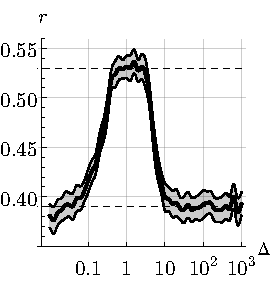
\includegraphics{imgs/2Drdel.pdf}
    % \hspace{5 mm} 
    \addletter{115}{c}
    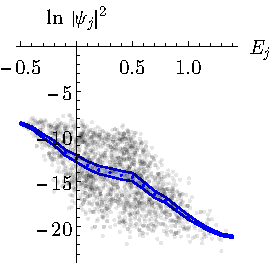
\includegraphics{imgs/2Dtherm_1.pdf}
    \caption{a) ... b) ... c) ... }
    \label{fig:2Dtherm}
\end{figure}


\begin{figure}[h]
    \centering
    \addletter{80}{a}
    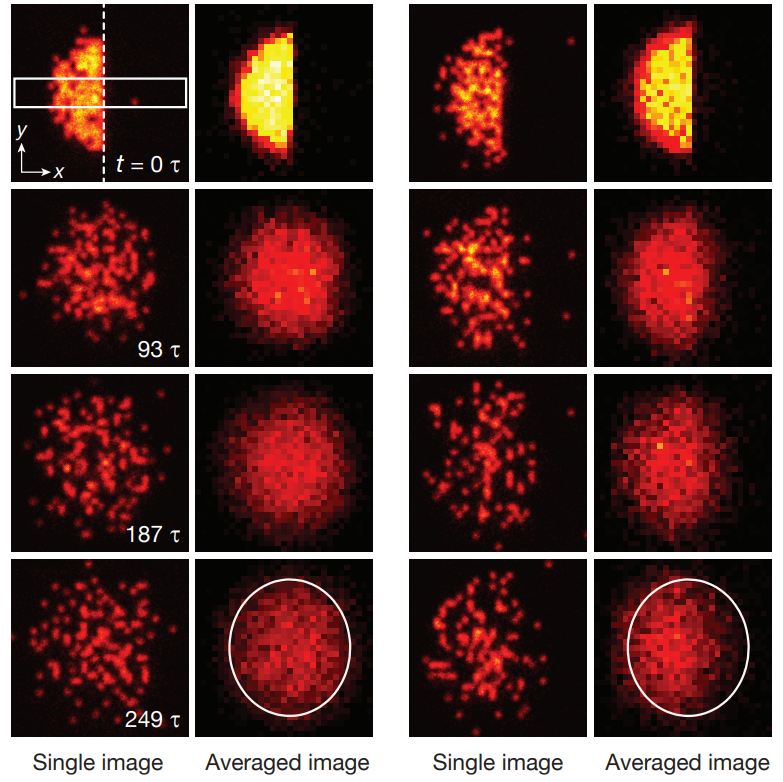
\includegraphics[align=c, width=0.33\textwidth]{imgs/MBL_2D_exp_1.png}
    \hspace{10 mm} 
    \addletter{80}{b}
    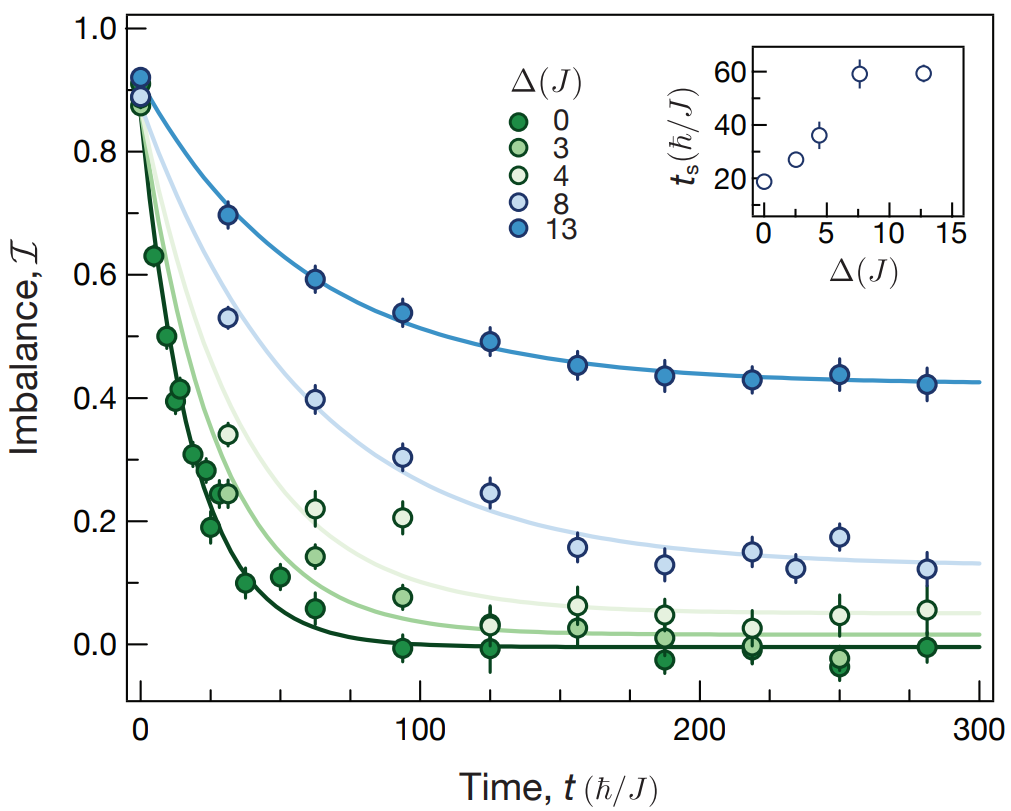
\includegraphics[align=c, width=0.4\textwidth]{imgs/MBL_2D_exp_2.png}
    % 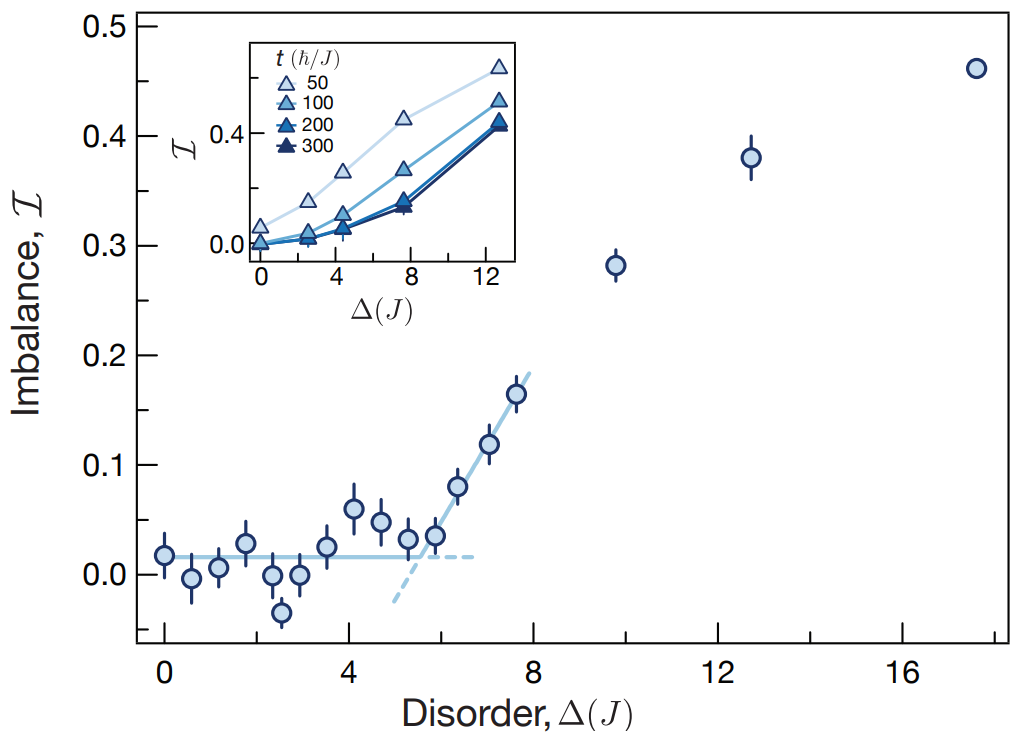
\includegraphics[align=c, width=0.4\textwidth]{imgs/MBL_2D_exp_3.png}
    \caption{
        a) Raw fluorescence images (red to yellow corresponds to increasing detected light level) showing the evolution of the initial density step without disorder \cite{Choi_2016} . 
        b) Relaxation dynamics of a density domain wall \cite{Choi_2016} .
    }
    \label{fig:loc2D1}
\end{figure}


% experimental implementation of the model